

\renewcommand{\thechapter}{A} 
\chapter{Parameters of Compact Binary Coalescences}
\label{Parameters_CBC_appendix}

This appendix provides a reference summary of the parameters used to describe a CBC system with quasi-circular orbits, following the conventions of \cite{likelihood_formula, GWTC4_introduction}. The parameters are grouped into mass, spin, tidal, and extrinsic categories; those employed in the injections and PE analyses of this work are indicated with $\star$.

\renewcommand{\arraystretch}{1.3}

{
\setlength{\LTleft}{0pt plus 1fill}
\setlength{\LTright}{0pt plus 1fill}
\begin{longtable}{lcp{9cm}}

\caption{Parameters describing a CBC system with quasi-circular orbits \cite{likelihood_formula, GWTC4_introduction}. Parameters used in this work are indicated with $\star$.}
\label{tab:CBC_parameters} \\

\hline\hline
\multicolumn{1}{c}{Parameter name} &
\multicolumn{1}{c}{Symbol} &
\multicolumn{1}{c}{Definition [Dimensions]} \\
\midrule
\endfirsthead

\multicolumn{3}{c}%
{{\tablename\ \thetable\ \textit{(continued)}}} \\

\hline\hline
\multicolumn{1}{c}{Parameter name} &
\multicolumn{1}{c}{Symbol} &
\multicolumn{1}{c}{Definition [Dimensions]} \\
\midrule
\endhead

\hline
\addlinespace[4pt]
\multicolumn{3}{c}{{\textit{Continued on next page}}} \\
\endfoot

\bottomrule
\endlastfoot

%------------------------------------------------
\addlinespace[5pt]
\multicolumn{3}{l}{\textit{\textbf{Mass parameters}}} \\
\hline
\addlinespace[5pt]

\, Primary/secondary mass & $m_1^\star,\,m_2^\star$ &
Mass of the more (less) massive component, $m_1\geq m_2$ $[M_\odot]$ \\

\, Chirp mass & $\mathcal{M}$ &
$\mathcal{M}=\eta^{3/5}M$ $[M_\odot]$ \\

\, Total mass & $M$ &
$M=m_1+m_2$ $[M_\odot]$ \\

\, Final mass & $M_f$ &
Mass of the remnant $[M_\odot]$ \\

\, Mass ratio & $q$ &
$q=m_2/m_1\leq 1$ [dimensionless] \\

\, Symmetric mass ratio & $\eta$ &
$\eta=m_1m_2/M^2\leq 1/4$ [dimensionless] \\

\, Radiated energy & $E_\mathrm{rad}$ &
$E_\mathrm{rad}=(M-M_f)c^2$ [energy] \\

%------------------------------------------------
\addlinespace[5pt]
\multicolumn{3}{l}{\textit{\textbf{Spin parameters}}} \\
\hline
\addlinespace[5pt]

\, Primary/secondary spin vectors & $\mathbf{S}_1,\,\mathbf{S}_2$ &
Spin angular momentum of the primary/secondary [ang. mom.] \\

\, Dimensionless spin magnitudes & $\chi_1^\star,\,\chi_2^\star$ &
$\chi_{1,2}=c|\mathbf{S}_{1,2}|/(Gm_{1,2}^2)\leq 1$ [dimensionless] \\

\, Remnant spin magnitude & $\chi_f$ &
$\chi_f=cS_f/(GM_f^2)\leq 1$  where $S_f$ is the magnitude of the remnant's spin
angular momentum [dimensionless] \\

\, Orbital ang. momentum & $\mathbf{L}$ &
Instantaneous orbital angular momentum about the center of mass [ang. mom.] \\

\, Total ang. momentum & $\mathbf{J}$ &
$\mathbf{J}=\mathbf{L}+\mathbf{S}_1+\mathbf{S}_2$ [ang. mom.] \\

\, Primary/secondary tilt angles & $\theta_1^\star,\,\theta_2^\star$ &
Angle between $\mathbf{S}_{1,2}$ and $\mathbf{L}$ [angle] \\

\, Spin azimuthal difference & $\phi_{12}^\star$ &
Angle between $\mathbf{L}\times(\mathbf{S}_1\times\mathbf{L})$ and $\mathbf{L}\times(\mathbf{S}_2\times\mathbf{L})$ [angle] \\

\, Effective inspiral spin & $\chi_\mathrm{eff}$ &
$(m_1\chi_{1z}+m_2\chi_{2z})/M$ [dimensionless] \\

\, Effective precession spin & $\chi_p$ &
Avg.\ over precession cycles \cite{effective_precession_spin} [dimensionless] \\

%------------------------------------------------
\multicolumn{3}{l}{\textit{\textbf{Tidal parameters}}} \\
\hline
\addlinespace[5pt]

\, Tidal deformabilities & $\Lambda_1,\,\Lambda_2$ &
Dimensionless tidal deformability; $\Lambda_{1,2}=0$ for BHs [dimensionless] \\

\, Effective tidal deformability & $\tilde{\Lambda}$ &
Dominant tidal combination; $\tilde{\Lambda}=0$ for BBH [dimensionless] \\

%------------------------------------------------
\multicolumn{3}{l}{\textit{\textbf{Extrinsic parameters}}} \\
\hline
\addlinespace[5pt]

\, Luminosity distance & $D_L^\star$ &
Distance to the source [Mpc] \\

\, Redshift & $z$ &
Computable from $D_L$ assuming a cosmological model [dimensionless] \\

\, Source inclination & $\theta_{JN}^\star$ &
Angle between $\mathbf{J}$ and line of sight $\mathbf{N}$ [angle] \\

\, Orbital inclination & $\iota$ &
Angle between $\mathbf{L}$ and $\mathbf{N}$ [angle] \\

\, Coalescence time & $t_c^\star$ &
GPS time at the geocenter [time] \\

\, Coalescence phase & $\phi_c^\star$ &
Orbital phase at coalescence [angle] \\

\, Right ascension & $\alpha^\star$ &
Celestial longitude [angle] \\

\, Declination & $\delta^\star$ &
Celestial latitude [angle] \\

\, Polarization angle & $\psi^\star$ &
Rotates polarizations in the plane orthogonal to propagation [angle] \\

\, Azimuthal spin angle & $\phi_{JL}^\star$ &
Angle between $\mathbf{J}$ and $\mathbf{L}$ projected on the sky plane [angle] \\
\end{longtable}
}



\renewcommand{\thechapter}{B} 
\chapter{Practical guide to HPC workflows}
\label{Reproducibility tutorial}

The motivation for including this appendix comes from the desire to make life easier for future students who will use the same tools, especially since many parts of this tutorial came with their fair share of headaches. It collects the day-to-day commands, configuration patterns, and troubleshooting notes accumulated while running the analyses of this thesis on two HPC clusters. It is not a repetition of the pipeline described in \S\ref{sec:automation_picasso}, but a practical reference for a student facing the same kind of environment for the first time. All pipeline-specific reproducibility details (configuration files, directory layout, job dependency logic) are documented in \S\ref{sec:automation_picasso} and Appendix~$\S$\ref{implementataion_pipeline}; the complete code is publicly available at \url{https://github.com/XxavierGarcia/TFM_reproducibility_material}.

\section{SSH access and aliases}

Both clusters are accessed via SSH (Secure Shell), a protocol that opens an encrypted terminal session on a remote machine: once connected, commands typed locally are executed directly on the cluster, as if sitting in front of it. On a Linux machine, an SSH client is available out of the box:

\begin{verbatim}
ssh username@picasso.scbi.uma.es
\end{verbatim}

(Users connecting from Windows Subsystem for Linux may need to append \texttt{-o KexAlgorithms=\allowbreak ecdh-sha2-nistp521} to this and every following \texttt{ssh}/\texttt{scp} command, since its older default OpenSSH client does not otherwise offer an algorithm accepted by Picasso's server; this flag is omitted from the rest of this tutorial.)

On CIT, the IGWN LDAS head nodes serve as the entry point (LIGO.ORG credentials required):

\begin{verbatim}
ssh username@ldas-grid.ligo.caltech.edu
\end{verbatim}

Typing these every time quickly becomes impractical. Two alternatives exist. The first is to define shell aliases in \texttt{\textasciitilde/.bashrc}:

\begin{verbatim}
alias picasso='ssh username@picasso.scbi.uma.es'
alias caltech='ssh username@ldas-grid.ligo.caltech.edu'
\end{verbatim}

Once these lines are added and the shell configuration is reloaded (\texttt{source \textasciitilde/.bashrc} or a new terminal), the full commands above are replaced by simply typing \texttt{picasso} or \texttt{caltech}.

The second, more robust option is to add entries to \texttt{\textasciitilde/.ssh/config}:

\begin{verbatim}
Host picasso
    HostName picasso.scbi.uma.es
    User username
    IdentityFile ~/.ssh/id_rsa
\end{verbatim}

With this configuration, \texttt{ssh picasso} and \texttt{scp picasso:path/file .} work directly.

\section{Remote editing with VS Code}

Editing files on the cluster through \texttt{nano} or \texttt{vim} works but is slow for larger scripts. VS Code's {Remote - SSH} extension provides a full graphical editor connected to the cluster filesystem:

\begin{enumerate}
  \item Install the \textit{Remote - SSH} extension from the VS Code marketplace.
  \item Open the command palette (\texttt{Ctrl+Shift+P}), type \textit{Remote-SSH: Connect to Host}, and select the host (or add a new one pointing to \texttt{picasso.scbi.uma.es}).
  \item Once connected, use \textit{File $\to$ Open Folder} to navigate to the working directory.
\end{enumerate}

This allows browsing the directory tree, viewing output figures directly, and editing configuration files without leaving the editor.

\section{Transferring files with \texttt{scp}}

\texttt{scp} (secure copy) transfers files between any two machines reachable via SSH. The basic syntax is \texttt{scp [options] source destination}, where either side can be \texttt{host:path}.

\begin{verbatim}
# Copy a single file from the local machine to the cluster
scp local_file.py username@picasso.scbi.uma.es:~/lenskyloc/

# Copy an entire directory (-r for recursive)
scp -r username@picasso.scbi.uma.es:~/lenskyloc/inj001/result/ .

# Transfer between two clusters (run from CIT)
scp -r username@picasso.scbi.uma.es:~/lenskyloc/pesummary_jsons .
\end{verbatim}

On CIT, the Jupyter interface (\url{https://jupyter.ligo.caltech.edu}) provides an alternative for downloading files: compress them first with \texttt{zip -r archive.zip directory/} and download the archive through the browser.

\section{Persistent terminal sessions with \texttt{screen}}

An SSH connection that drops (timeout, laptop closing, network change) kills any process running inside it. The \texttt{screen} utility creates a persistent terminal session on the cluster that survives disconnections:

\begin{verbatim}
screen -S analysis         # create a named session
# ... run any long command ...
# detach: Ctrl+a, then d
screen -ls                 # list active sessions
screen -r analysis         # reattach
exit                       # close the session permanently
\end{verbatim}

This is essential for interactive tasks that take more than a few minutes (monitoring logs, running quick post-processing scripts) but are not worth submitting as batch jobs.

\section{Conda environments}

Both clusters use \texttt{conda} environments to manage Python dependencies. On Picasso, the analysis environment was created and maintained manually:

\begin{verbatim}
conda create -n hanabi_bilby260 python=3.10
conda activate hanabi_bilby260
pip install bilby bilby_pipe hanabi lalsuite dynesty ...
\end{verbatim}

The activation line is included in every generated SLURM script, so each job runs in the correct environment automatically. On CIT, the \texttt{igwn} environment distributed via CVMFS is activated directly instead.

When the home directory quota on Picasso fills up (check with \texttt{quota}), the most effective remedy is to clear the conda cache, which accumulates downloaded packages and can grow to several gigabytes:

\begin{verbatim}
conda clean --all
\end{verbatim}

\section{SLURM: submitting and monitoring jobs on Picasso}

Picasso uses the SLURM workload manager. Jobs are submitted with \texttt{sbatch}, monitored with \texttt{squeue}, and cancelled with \texttt{scancel}:

\begin{verbatim}
sbatch job_script.sh           # submit a job
squeue -u username             # list your running/pending jobs
scancel JOB_ID                 # cancel one job
scancel --user username        # cancel all your jobs
\end{verbatim}

A typical SLURM header for a single-image PE job in this thesis (\S\ref{sec:bilby_config}) looks like:

\begin{verbatim}
#!/bin/bash
#SBATCH --job-name=lenskyloc_inj_001_img1
#SBATCH --cpus-per-task=128
#SBATCH --mem=110G
#SBATCH --time=48:00:00
#SBATCH --constraint=cal

export MPLCONFIGDIR=$LOCALSCRATCH/$USER
conda activate hanabi_bilby260
\end{verbatim}

The \texttt{-{}-constraint=cal} flag restricts the job to nodes of a specific hardware class; \texttt{MPLCONFIGDIR} is redirected to the node-local scratch space to avoid \texttt{matplotlib} cache errors on compute nodes whose home filesystem is read-only.

For dependent jobs (e.g.\ a joint analysis that must wait for both single-image jobs), SLURM's \texttt{-{}-dependency} flag is used:

\begin{verbatim}
JOB1=$(sbatch img1.sh | awk '{print $4}')
JOB2=$(sbatch img2.sh | awk '{print $4}')
sbatch --dependency=afterok:$JOB1:$JOB2 joint.sh
\end{verbatim}

To monitor a running job's progress in real time, inspect the sampler log:

\begin{verbatim}
tail -f log_data_analysis/*.err
\end{verbatim}

If a job is killed by the wall-time limit, it can be resubmitted and will resume from the last \texttt{Dynesty} checkpoint (written every 30 minutes by default via \texttt{check\_point\_delta\_t=1800}).

\section{HTCondor: submitting and monitoring jobs on CIT}

CIT uses HTCondor instead of SLURM. The analogous commands are:

\begin{verbatim}
condor_submit file.submit      # submit a job
condor_q                       # list your running/pending jobs
condor_rm JOB_ID               # cancel one job
condor_q -hold                 # diagnose jobs stuck in "held" state
\end{verbatim}

One common pitfall: HTCondor requires the executable specified in the \texttt{.submit} file to have the Unix execute permission. If a \texttt{.sh} script submitted as \texttt{executable} produces \texttt{errno=13: Permission denied}, the fix is:

\begin{verbatim}
chmod +x script.sh
\end{verbatim}

The permissions can be verified with \texttt{ls -l}: the file should show \texttt{-rwxr-xr-x} (the \texttt{x} flags) rather than \texttt{-rw-r-{}-r-{}-}.

\section{Useful everyday commands}

The following commands were used daily throughout this project:

\begin{center}
\renewcommand{\arraystretch}{1.2}
\begin{tabular}{ll}
\hline\hline
\textbf{Task} & \textbf{Command} \\
\hline
Search for a string inside a file & \texttt{grep pattern file} \\
Compare two files line by line & \texttt{diff file1 file2} \\
Check the size of a file or directory & \texttt{du -sh path} \\
Check sizes of everything in home & \texttt{du -sh \textasciitilde/*} \\
Jump to the end of a large file & \texttt{less file}, then \texttt{Shift+G} \\
View the last/first lines of a log & \texttt{tail -n 50 file} / \texttt{head -n 50 file} \\
Check available disk quota (Picasso) & \texttt{quota} \\
See all options of a command & \texttt{command -{}-help} \\
\hline
\end{tabular}
\end{center}

\section{Troubleshooting summary}

The most common issues encountered during this project, and their solutions:

\begin{itemize}
  \item \textbf{Wall-time kills on Picasso:} resubmit the same script; \texttt{Dynesty} resumes from the latest checkpoint. This was also the mechanism that limited the last seven joint analyses when the allocation dropped to 24\,h (\S\ref{sec:incomplete_events}).
  \item \textbf{Matplotlib cache errors on compute nodes:} redirect \texttt{MPLCONFIGDIR} to node-local scratch (already included in the SLURM headers above).
  \item \textbf{PESummary failing on Picasso:} the version available in the Picasso environment produced errors; the workaround was to run the summary-page and sky-map generation on CIT instead, where the \texttt{igwn} environment handles it correctly (\S\ref{sec:automation_picasso}).
  \item \textbf{HTCondor ``held'' jobs on CIT:} diagnose with \texttt{condor\_q -hold}; the most frequent cause was a missing execute permission on the \texttt{.sh} script (see above).
  \item \textbf{Home directory quota full on Picasso:} run \texttt{conda clean -{}-all} to free cached packages.
\end{itemize}

\section{Additional resources}
\begin{itemize}
  \item SLURM documentation: \url{https://slurm.schedmd.com/documentation.html}
  \item HTCondor documentation: \url{https://htcondor.readthedocs.io/en/latest/}
  \item Picasso user guide (SCBI): \url{https://www.scbi.uma.es/site/}
  \item IGWN Computing Guide (CIT access): \url{https://computing.docs.ligo.org/guide/}
  \item Complete pipeline code: \url{https://github.com/XxavierGarcia/TFM_reproducibility_material}
\end{itemize}



\renewcommand{\thechapter}{C} 
\chapter{Detailed implementation of the pipeline}
\label{implementataion_pipeline}

This appendix reproduces two representative \texttt{.ini} configuration files generated automatically by \texttt{Generator\_inis\_lenskyloc.py} (\S\ref{sec:automation_picasso}) for event \texttt{inj001}: the single-image configuration for image 1 (\S\ref{sec:bilby_config}), and the joint configuration combining both images (\S\ref{sec:hanabi_joint}). The complete pipeline code, including both the Picasso (SLURM) and CIT (HTCondor) branches described in \S\ref{sec:automation_picasso}, is publicly available at the GitHub repository listed in Appendix~$\S$\ref{Reproducibility tutorial}.

\section{Single-image configuration}
\label{app:single_ini_example}

\begin{lstlisting}[style=numpyStyle, caption={Single-image configuration file for image 1 of event \texttt{inj001}.}, label={lst:single_ini_example}]

#################################################
## Data generation arguments
#################################################
trigger-time=1268585121.2749617
gaussian-noise=True
zero-noise=False

##################################################
## Detector arguments
##################################################
detectors=[H1, L1]
duration=4 
psd-dict={"H1": "/mnt/home/users/uib54_res/resh000464/noise_curves/T2500310-v2_O5a_strain_psd.txt", "L1": "/mnt/home/users/uib54_res/resh000464/noise_curves/T2500310-v2_O5a_strain_psd.txt"} 
sampling-frequency=2048
reference-frequency=20
minimum-frequency={'H1': 20, 'L1': 20, 'waveform':13.33}
maximum-frequency= {'H1': 896, 'L1': 896}

##################################################
## Injection arguments
##################################################
injection=True
injection-dict={'mass_1': 68.50715378171094, 'mass_2': 40.35264268122141, 'luminosity_distance': 2889.5612112115464, 'a_1': 0.4527593183131344, 'a_2': 0.5997569914138758, 'tilt_1': 1.4148137284549118, 'tilt_2': 1.685673833551925, 'phi_12': 1.2201031723904865, 'phi_jl': 3.7845775009109737, 'theta_jn': 0.5351550350716038, 'psi': 2.351204394088696, 'phase': 4.596028055035042, 'geocent_time': 1268585121.2749617, 'ra': 6.094792612884527, 'dec': -0.6855988520635732, 'minimum_frequency': 20.0, 'reference_frequency': 20.0, 'image_type': 1.0} 
injection-waveform-approximant=IMRPhenomXPNR
injection-frequency-domain-source-model=hanabi.lensing.waveform.strongly_lensed_BBH_waveform
injection-waveform-arguments={'reference_frequency': 20, 'minimum_frequency': 20, 'pn_amplitude_order': 0}

##################################################
## Job submission arguments
##################################################
label=lenskyloc_inj_001_hanabi_single_img1
outdir=/mnt/home/users/uib54_res/resh000464/lenskyloc/lenskyloc_runs/inj001/inj001_img1
request-disk=6.0
request-memory=110.0
request-memory-generation=2.0
request-cpus=128
scheduler=slurm
scheduler-args=constraint=cal
extra-lines=export MPLCONFIGDIR=$LOCALSCRATCH/$USER
scheduler-analysis-time=48:00:00

##################################################
## Output arguments
##################################################
result-format=json

##################################################
## Prior arguments
##################################################
prior-dict={chirp-mass: bilby.gw.prior.UniformInComponentsChirpMass(minimum=31.819, maximum=59.093, name='chirp_mass', boundary=None),
    mass-ratio: bilby.gw.prior.UniformInComponentsMassRatio(minimum=0.05, maximum=1.0, name='mass_ratio', latex_label='$q$', unit=None, boundary=None),
    mass-1: Constraint(minimum=5.0, maximum=200.0, name='mass_1', latex_label='$m_1$', unit=None),
    mass-2: Constraint(minimum=5.0, maximum=200, name='mass_2', latex_label='$m_2$', unit=None),
    a-1: Uniform(minimum=0, maximum=0.99, name='a_1', latex_label='$a_1$', unit=None, boundary=None),
    a-2: Uniform(minimum=0, maximum=0.99, name='a_2', latex_label='$a_2$', unit=None, boundary=None),
    tilt-1: Sine(minimum=0, maximum=3.141592653589793, name='tilt_1'),
    tilt-2: Sine(minimum=0, maximum=3.141592653589793, name='tilt_2'),
    phi-12: Uniform(minimum=0, maximum=6.283185307179586, name='phi_12', boundary='periodic'),
    phi-jl: Uniform(minimum=0, maximum=6.283185307179586, name='phi_jl', boundary='periodic'),
    luminosity-distance: Uniform(minimum=50, maximum=20000, name='luminosity_distance', latex_label='$d_L$', unit='Mpc', boundary=None),
    cos-theta-jn: Uniform(minimum=-1, maximum=1, name='cos_theta_jn', latex_label='$\cos\theta_{JN}$', unit=None, boundary=None),
    psi: Uniform(minimum=0, maximum=3.141592653589793, name='psi', boundary='periodic'),
    phase: Uniform(minimum=0, maximum=6.283185307179586, name='phase', boundary='periodic'),
    dec: Cosine(minimum=-1.5707963267948966, maximum=1.5707963267948966, name='dec', latex_label='$\mathrm{DEC}$', unit=None, boundary=None),
    ra: Uniform(minimum=0, maximum=6.283185307179586, name='ra', latex_label='$\mathrm{RA}$', unit=None, boundary='periodic'),
    image_type = 1.0}

##################################################
## Sampler arguments
##################################################
n-parallel=3
sampler-kwargs={'nlive': 1000, 'naccept': 60, 'check_point_plot': True, 'check_point_delta_t': 1800, 'print_method': 'interval-60', 'sample': 'acceptance-walk', 'samples': 'acceptance-walk', 'npool': 128}
distance_marginalization=False
time-marginalization=False
phase-marginalization=False

###################################################
## Waveform arguments (used for the analysis)
###################################################
waveform-generator=bilby.gw.waveform_generator.WaveformGenerator
frequency-domain-source-model=hanabi.lensing.waveform.strongly_lensed_BBH_waveform
waveform-approximant=IMRPhenomXPNR
enforce-signal-duration=False
catch-waveform-errors=True
pn-amplitude-order=1
\end{lstlisting}

The injection uses \texttt{pn\_amplitude\_order=0} while the analysis uses \texttt{pn-amplitude-order=1}. This argument, inherited from the PN waveform families supported by \textsc{LALSimulation}, is not used by the phenomenological \texttt{IMRPhenomXPNR} model to construct its amplitude: generating the same waveform with \texttt{pn\_amplitude\_order} set to $0$ and to $1$, keeping all other parameters fixed, leaves the frequency-domain strain unchanged. This configuration mismatch is therefore a leftover setting from the template with no real effect on the results of this thesis.


\newpage
\section{Joint configuration}
\label{app:joint_ini_example}

\begin{lstlisting}[style=numpyStyle, caption={Joint configuration file for event \texttt{inj001}.}, label={lst:joint_ini_example}]
###################################################
## Job submission arguments
###################################################
label=lenskyloc_inj_001_hanabi_joint
outdir=/mnt/home/users/uib54_res/resh000464/lenskyloc/lenskyloc_runs/inj001/inj001_joint
request-disk=6.0
request-memory=180.0 
request-memory-generation=2.0
request-cpus=128
scheduler=slurm
scheduler-args=constraint=cal
extra-lines=export MPLCONFIGDIR=$LOCALSCRATCH/$USER
scheduler-analysis-time=71:30:00

###################################################
## Output arguments
###################################################
result-format=json

###################################################
## Sampler arguments
###################################################
sampler=dynesty
n-parallel=3
sampler-kwargs={'nlive': 1000, 'naccept': 60, 'check_point_plot': True, 'check_point_delta_t': 1800, 'print_method': 'interval-60', 'sample': 'acceptance-walk', 'samples': 'acceptance-walk', 'npool': 128}

###################################################
## Joint input arguments
###################################################
n-triggers=2
trigger-ini-files=[/mnt/home/users/uib54_res/resh000464/lenskyloc/lenskyloc_runs/inj001/single_event_001_image1.ini, /mnt/home/users/uib54_res/resh000464/lenskyloc/lenskyloc_runs/inj001/single_event_001_image2.ini]

###################################################
## Lensing prior argument
###################################################
common-parameters=[chirp_mass, mass_ratio, mass_1, mass_2, a_1, a_2, tilt_1, tilt_2, phi_12, phi_jl, cos_theta_jn, ra, dec, psi, phase]
lensing-prior-dict={relative-magnification^(1): 1, image_type^(1) = hanabi.lensing.prior.DiscreteUniform(name='image_type^(1)', minimum=1, N=3), relative_magnification^(2) = 1, image_type^(2) = hanabi.lensing.prior.DiscreteUniform(name='image_type^(2)', minimum=1, N=3)}


\end{lstlisting}

Figures~\ref{fig:pipeline_picasso} and \ref{fig:pipeline_cit} lay out, script by script, the two branches of the pipeline introduced in \S\ref{sec:automation_picasso}: the SLURM job generation and submission chain running on Picasso, and the HTCondor post-processing chain running on CIT.

%\begin{landscape}
%\begin{figure}[p]
    %\centering
    %\includegraphics[width=\linewidth]{Figures/pipeline_picasso_full.pdf}
    %\caption{Detailed implementation of the Picasso (SLURM) branch of the pipeline, including intermediate files and job scripts, referenced in \S\ref{sec:automation_picasso}.}
    %\label{fig:pipeline_picasso_full}
%\end{figure}
%\end{landscape}

%\begin{landscape}
%\begin{figure}[p]
    %\centering
    %\includegraphics[width=\linewidth]{Figures/pipeline_cit_full.pdf}
    %\caption{Detailed implementation of the CIT (HTCondor) post-processing branch, referenced in \S\ref{sec:automation_picasso} and \S\ref{sec:skymap_generation}.}
    %\label{fig:pipeline_cit_full}
%\end{figure}
%\end{landscape}


\begin{figure}[h!]
    \centering
    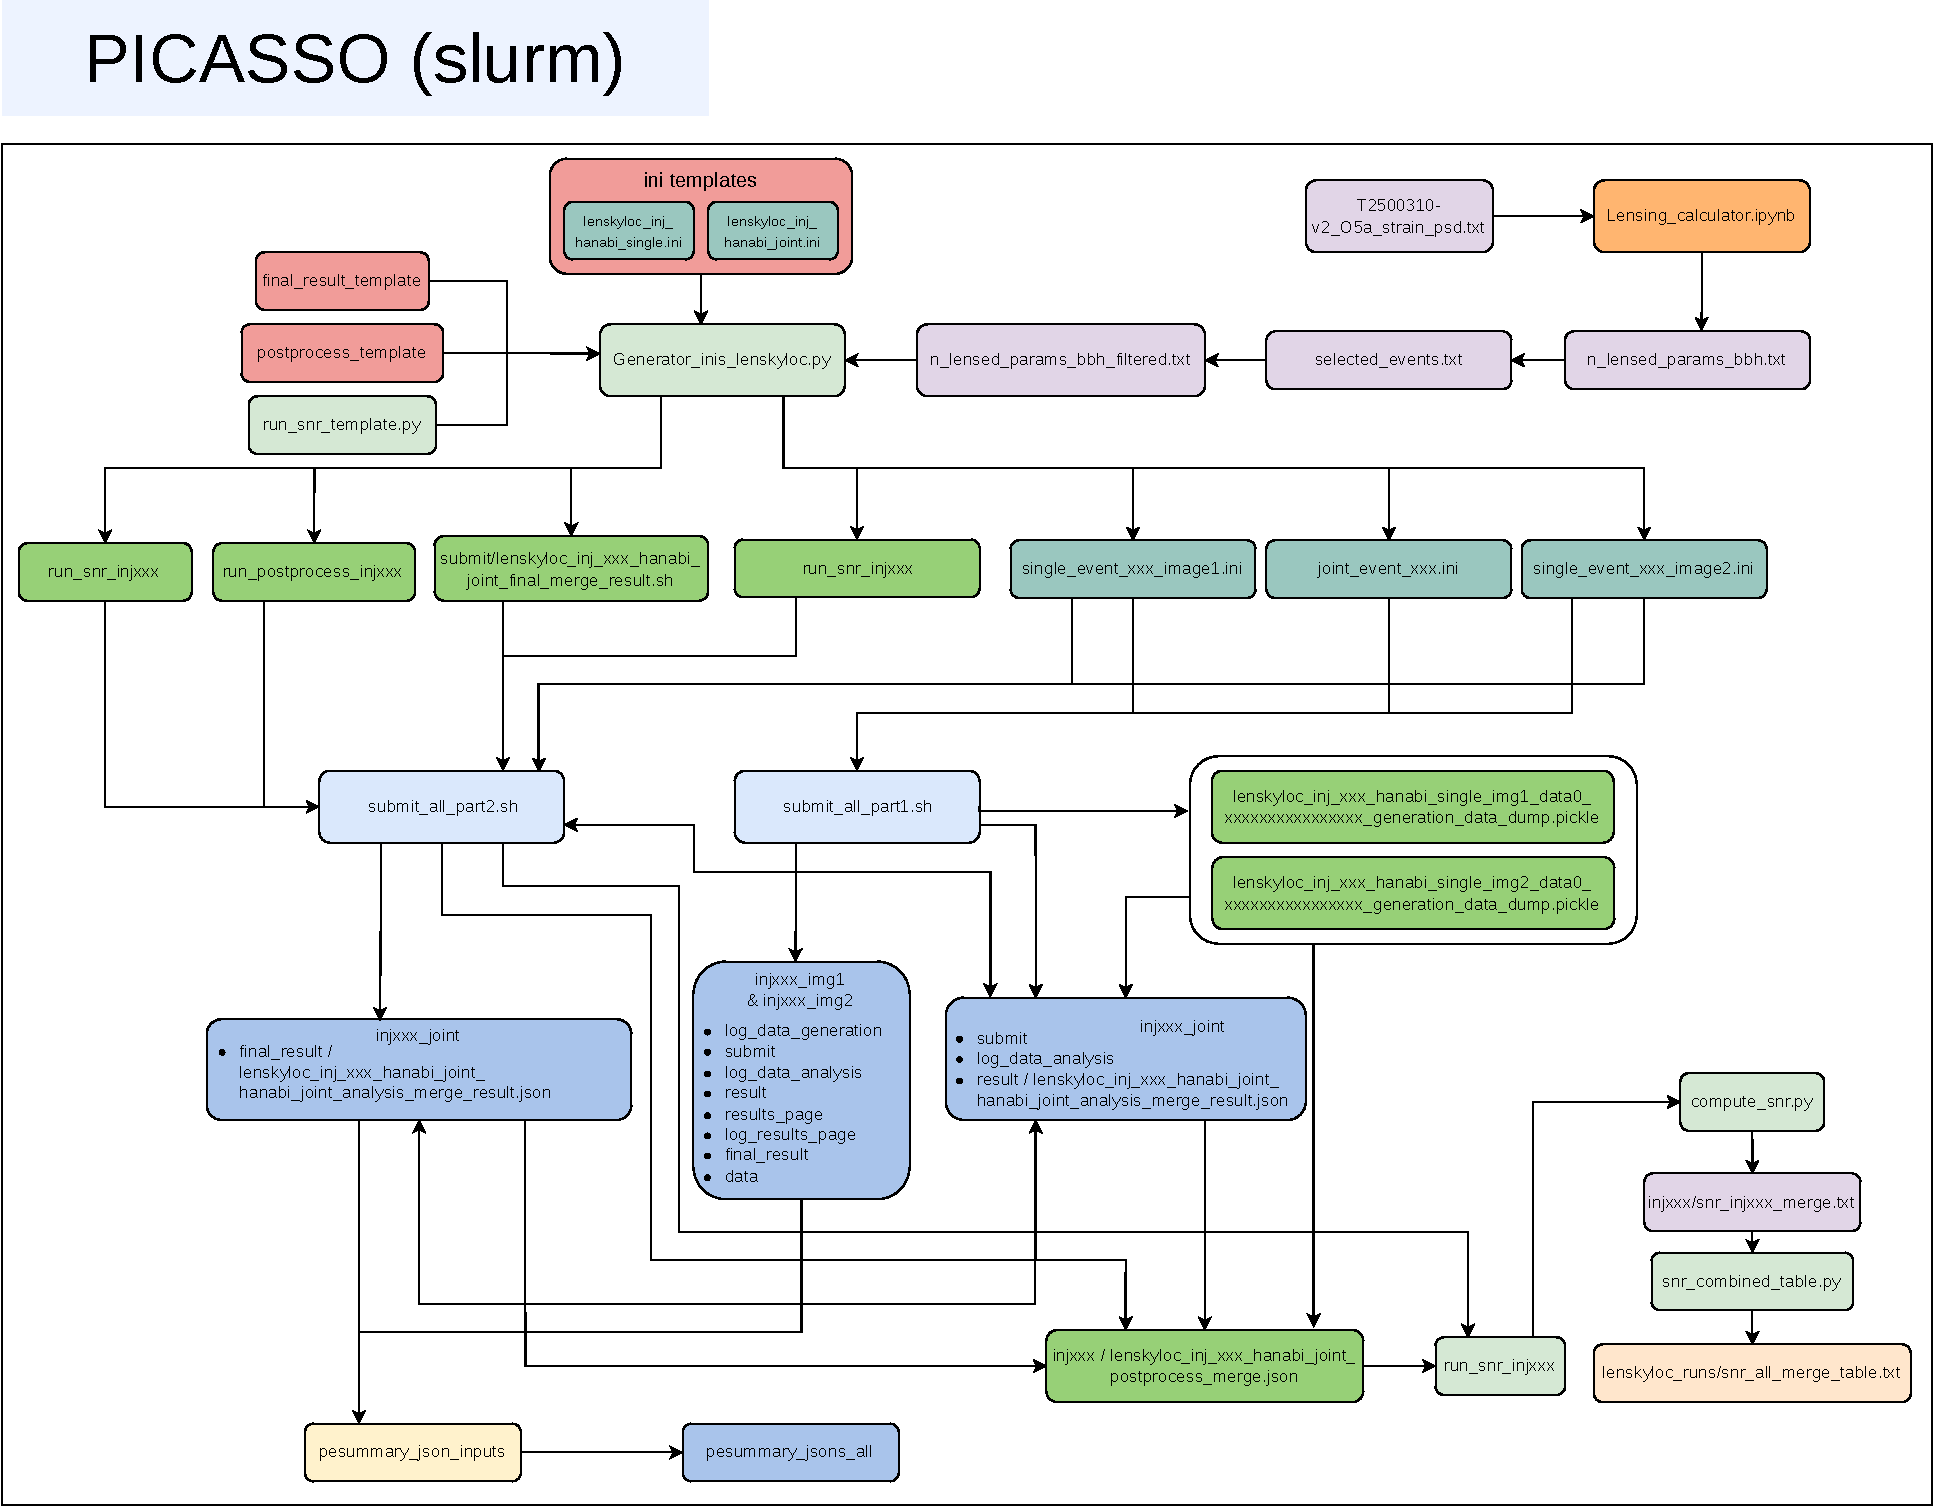
\includegraphics[width=\linewidth]{Figures/diagrama_pipeline_picasso.drawio.pdf}
    \caption[Detailed implementation of the Picasso branch of the pipeline]{Detailed implementation of the Picasso (SLURM) branch of the pipeline, referenced in \S\ref{sec:automation_picasso}. Best viewed digitally, zoomed in. An interactive version with clickable links to each script is available at \url{https://github.com/XxavierGarcia/TFM_reproducibility_material/blob/main/diagrama_pipeline.drawio.pdf} (download to enable links).}
    \label{fig:pipeline_picasso}
\end{figure}

\newpage

\begin{figure}[h!]
    \centering
    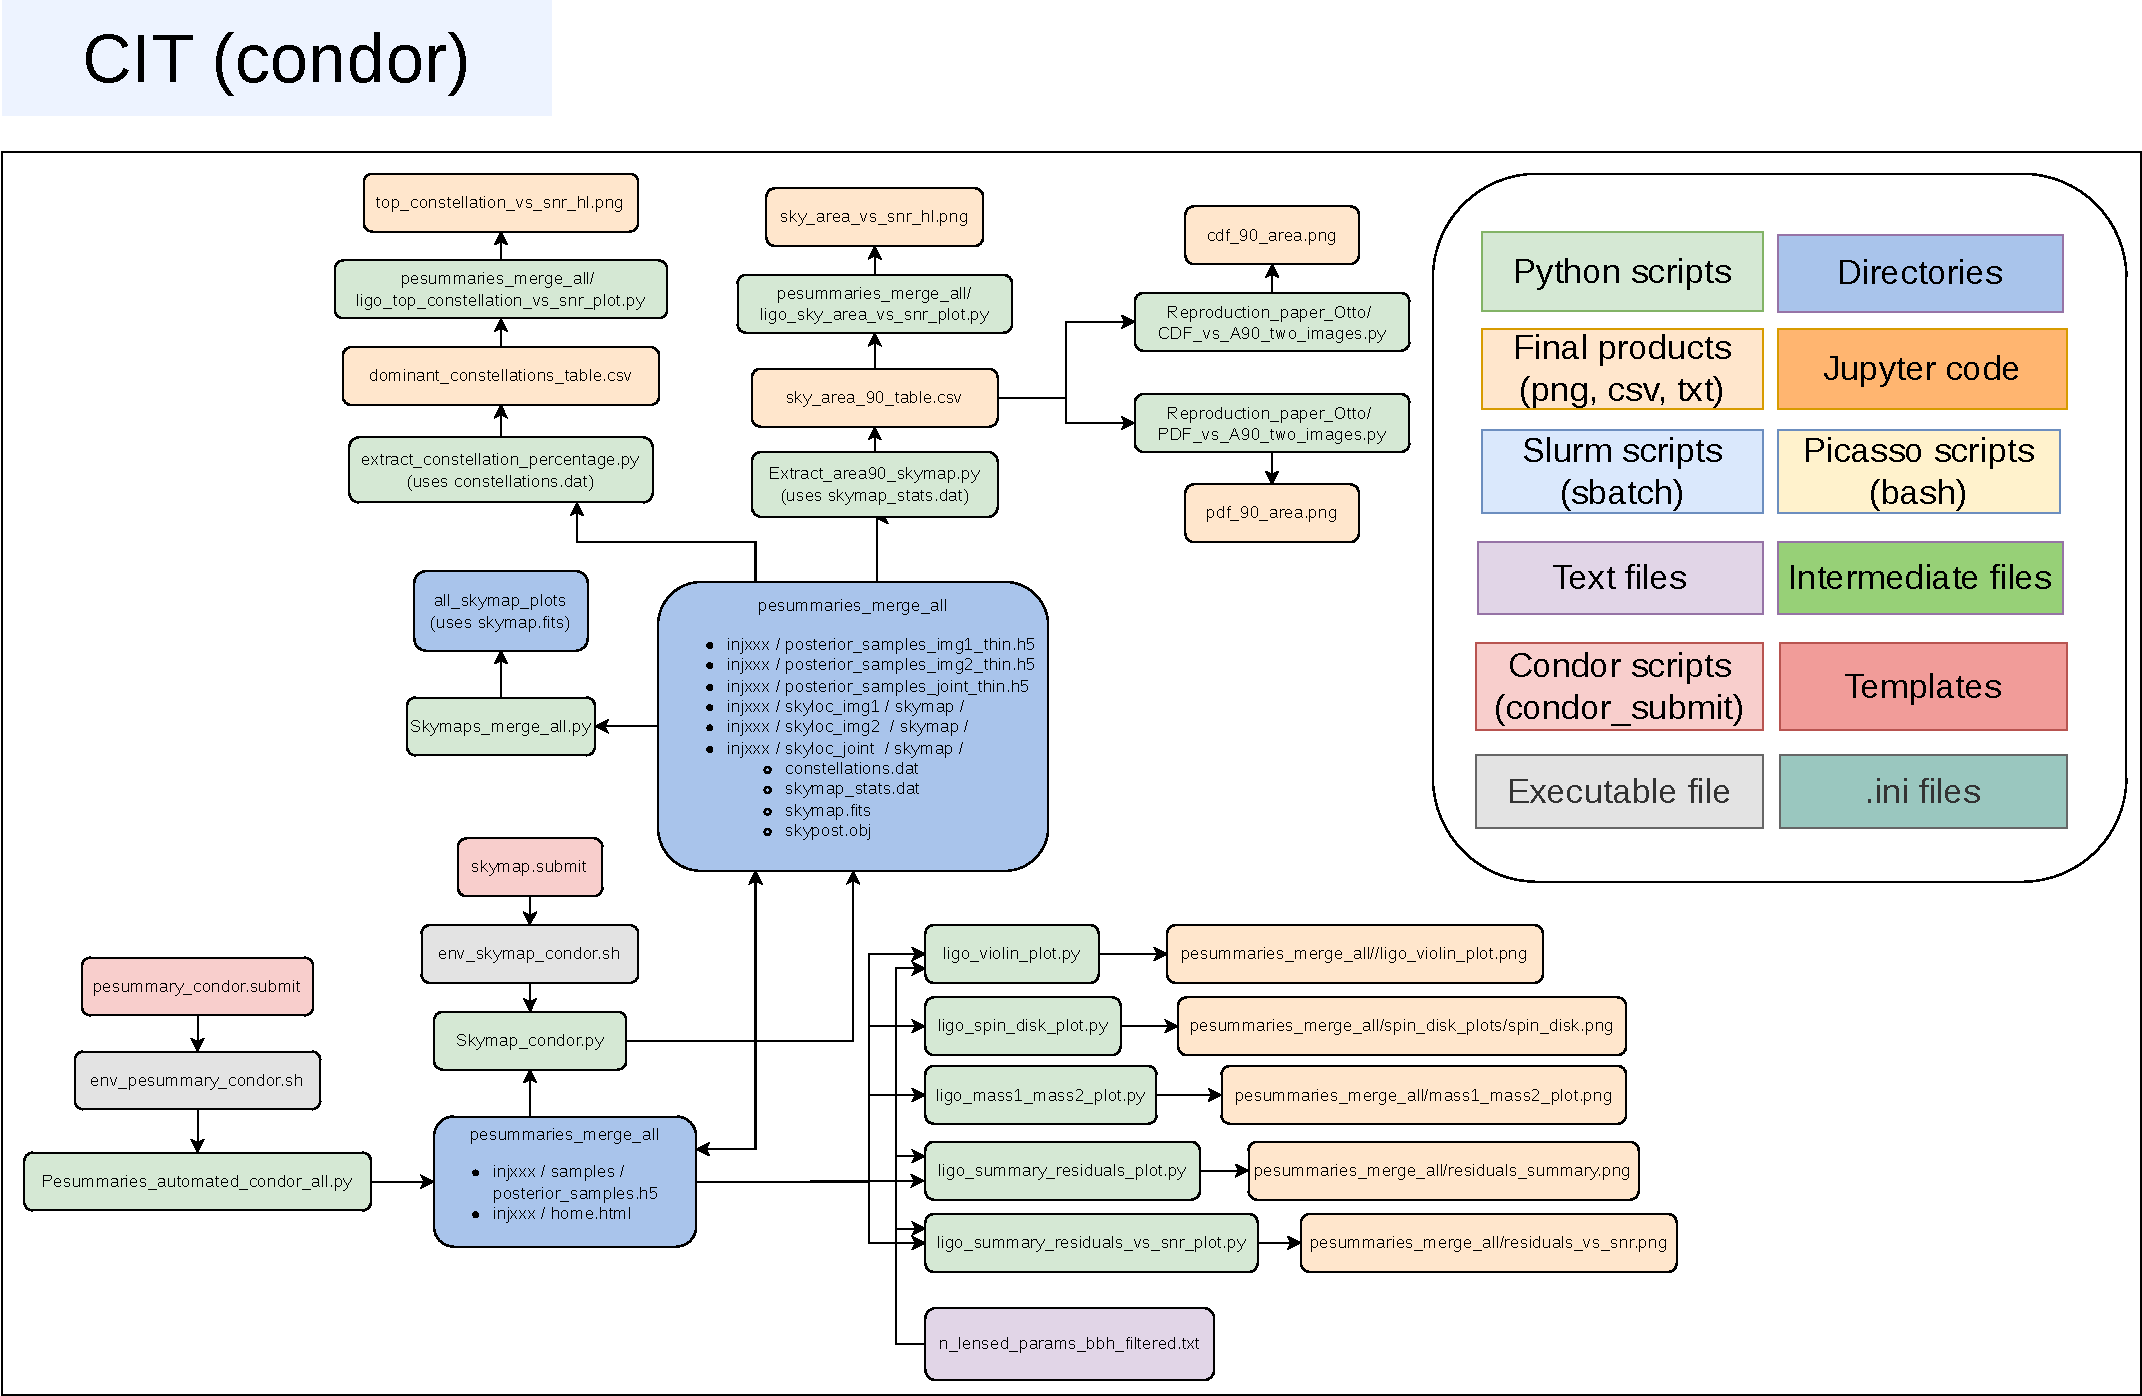
\includegraphics[width=\linewidth]{Figures/diagrama_pipeline_CIT.drawio.pdf}
    \caption[Detailed implementation of the CIT branch of the pipeline]{Detailed implementation of the CIT (HTCondor) post-processing branch of the pipeline, referenced in \S\ref{sec:automation_picasso} and \S\ref{sec:skymap_generation}. Best viewed digitally, zoomed in. An interactive version with clickable links to each script is available at \url{https://github.com/XxavierGarcia/TFM_reproducibility_material/blob/main/diagrama_pipeline.drawio.pdf} (download to enable links).}
    \label{fig:pipeline_cit}
\end{figure}



